% Unidades productivas de elaboración de productos de panadería por
% departamento. Adaptado de MDPyEP (2023), Tabla 9 (fuente original: SIIP,
% procesado por DGAPIyEP). Valores sin modificar.
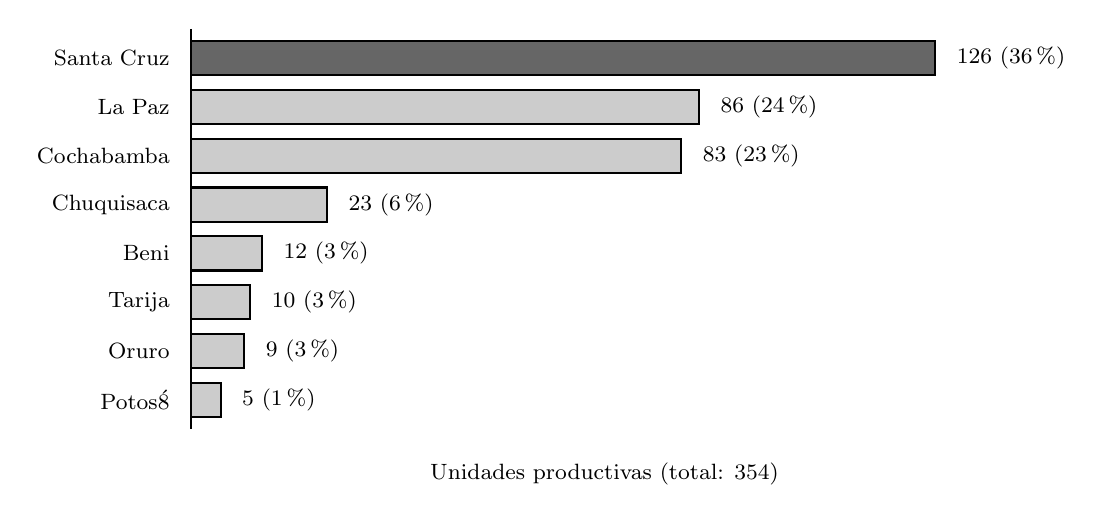
\begin{tikzpicture}[
    x=0.075cm,
    y=-0.62cm,
    barra/.style={draw, fill=black!20, thick},
    destacada/.style={draw, fill=black!60, thick},
    etiqueta/.style={font=\footnotesize, anchor=east},
    valor/.style={font=\footnotesize, anchor=west}
]

% Departamento / unidades productivas / participación
\foreach \dep/\val/\por [count=\i] in {
    Santa Cruz/126/36,
    La Paz/86/24,
    Cochabamba/83/23,
    Chuquisaca/23/6,
    Beni/12/3,
    Tarija/10/3,
    Oruro/9/3,
    Potosí/5/1}
{
    \ifnum\i=1
        \draw[destacada] (0,\i-0.35) rectangle (\val,\i+0.35);
    \else
        \draw[barra] (0,\i-0.35) rectangle (\val,\i+0.35);
    \fi
    \node[etiqueta] at (-2,\i) {\dep};
    \node[valor] at (\val+2,\i) {\val\ (\por\,\%)};
}

% Eje
\draw[thick] (0,0.4) -- (0,8.6);
\node[font=\footnotesize, anchor=north] at (70,9.1)
    {Unidades productivas (total: 354)};

\end{tikzpicture}
